%=====================================================
\begin{frame}{3.2.4. Данные по вопросам, включенным в блок ``Фактический уровень вертикального доверия'' }

\tiny

\begin{tabular}{lccl}

 & Раз в месяц  & Один раз в  &\\
 & или чаще    & полугодие  &\\
 &      &  или реже &\\

\begin{minipage}{0.5\textwidth}
Б15.  ``Как часто Вы лично за последний учебный год по своей инициативе обращались (обсуждали, советовались) по вопросам преподавания и воспитания конкретных обучающихся (воспитанников) или классов (групп) к директору (заведующему)?''
\end{minipage}
& \valCBDyesNumA & \valCBDnoNumA &
\begin{minipage}{1.55cm}
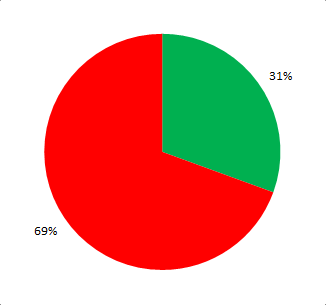
\includegraphics[width=1.5cm, height=1.5cm]{diag.png}
\end{minipage}
\\[0.7cm]

\begin{minipage}{0.5\textwidth}
Б16. ``Как часто Вы лично за последний учебный год по своей инициативе обращались (обсуждали, советовались) по вопросам преподавания и воспитания конкретных обучающихся (воспитанников) или классов (групп) к зам. директора (заведующего)?''
\end{minipage}
& \valCBDyesNumB & \valCBDnoNumB &
\begin{minipage}{1.55cm}
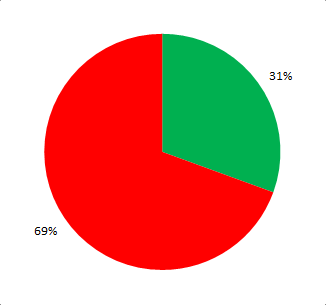
\includegraphics[width=1.5cm, height=1.5cm]{diag.png}
\end{minipage}
\\[0.7cm]

\begin{minipage}{0.5\textwidth}
Б17. ``Как часто Вы лично за последний учебный год по своей инициативе обращались (советовались, обсуждали) по вопросам преподавания и воспитания конкретных обучающихся (воспитанников) или классов (групп)  к заведующим кафедрами  (методобъединений, отделений)?''
\end{minipage}
& \valCBDyesNumC & \valCBDnoNumC &
\begin{minipage}{1.55cm}
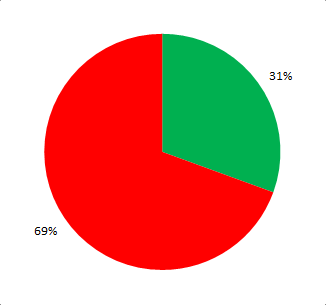
\includegraphics[width=1.5cm, height=1.5cm]{diag.png}
\end{minipage}
\\

\end{tabular}


\end{frame}


